\documentclass[1p]{elsarticle_modified}
%\bibliographystyle{elsarticle-num}

%\usepackage[colorlinks]{hyperref}
%\usepackage{abbrmath_seonhwa} %\Abb, \Ascr, \Acal ,\Abf, \Afrak
\usepackage{amsfonts}
\usepackage{amssymb}
\usepackage{amsmath}
\usepackage{amsthm}
\usepackage{scalefnt}
\usepackage{amsbsy}
\usepackage{kotex}
\usepackage{caption}
\usepackage{subfig}
\usepackage{color}
\usepackage{graphicx}
\usepackage{xcolor} %% white, black, red, green, blue, cyan, magenta, yellow
\usepackage{float}
\usepackage{setspace}
\usepackage{hyperref}

\usepackage{tikz}
\usetikzlibrary{arrows}

\usepackage{multirow}
\usepackage{array} % fixed length table
\usepackage{hhline}

%%%%%%%%%%%%%%%%%%%%%
\makeatletter
\renewcommand*\env@matrix[1][\arraystretch]{%
	\edef\arraystretch{#1}%
	\hskip -\arraycolsep
	\let\@ifnextchar\new@ifnextchar
	\array{*\c@MaxMatrixCols c}}
\makeatother %https://tex.stackexchange.com/questions/14071/how-can-i-increase-the-line-spacing-in-a-matrix
%%%%%%%%%%%%%%%

\usepackage[normalem]{ulem}

\newcommand{\msout}[1]{\ifmmode\text{\sout{\ensuremath{#1}}}\else\sout{#1}\fi}
%SOURCE: \msout is \stkout macro in https://tex.stackexchange.com/questions/20609/strikeout-in-math-mode

\newcommand{\cancel}[1]{
	\ifmmode
	{\color{red}\msout{#1}}
	\else
	{\color{red}\sout{#1}}
	\fi
}

\newcommand{\add}[1]{
	{\color{blue}\uwave{#1}}
}

\newcommand{\replace}[2]{
	\ifmmode
	{\color{red}\msout{#1}}{\color{blue}\uwave{#2}}
	\else
	{\color{red}\sout{#1}}{\color{blue}\uwave{#2}}
	\fi
}

\newcommand{\Sol}{\mathcal{S}} %segment
\newcommand{\D}{D} %diagram
\newcommand{\A}{\mathcal{A}} %arc


%%%%%%%%%%%%%%%%%%%%%%%%%%%%%5 test

\def\sl{\operatorname{\textup{SL}}(2,\Cbb)}
\def\psl{\operatorname{\textup{PSL}}(2,\Cbb)}
\def\quan{\mkern 1mu \triangleright \mkern 1mu}

\theoremstyle{definition}
\newtheorem{thm}{Theorem}[section]
\newtheorem{prop}[thm]{Proposition}
\newtheorem{lem}[thm]{Lemma}
\newtheorem{ques}[thm]{Question}
\newtheorem{cor}[thm]{Corollary}
\newtheorem{defn}[thm]{Definition}
\newtheorem{exam}[thm]{Example}
\newtheorem{rmk}[thm]{Remark}
\newtheorem{alg}[thm]{Algorithm}

\newcommand{\I}{\sqrt{-1}}
\begin{document}

%\begin{frontmatter}
%
%\title{Boundary parabolic representations of knots up to 8 crossings}
%
%%% Group authors per affiliation:
%\author{Yunhi Cho} 
%\address{Department of Mathematics, University of Seoul, Seoul, Korea}
%\ead{yhcho@uos.ac.kr}
%
%
%\author{Seonhwa Kim} %\fnref{s_kim}}
%\address{Center for Geometry and Physics, Institute for Basic Science, Pohang, 37673, Korea}
%\ead{ryeona17@ibs.re.kr}
%
%\author{Hyuk Kim}
%\address{Department of Mathematical Sciences, Seoul National University, Seoul 08826, Korea}
%\ead{hyukkim@snu.ac.kr}
%
%\author{Seokbeom Yoon}
%\address{Department of Mathematical Sciences, Seoul National University, Seoul, 08826,  Korea}
%\ead{sbyoon15@snu.ac.kr}
%
%\begin{abstract}
%We find all boundary parabolic representation of knots up to 8 crossings.
%
%\end{abstract}
%\begin{keyword}
%    \MSC[2010] 57M25 
%\end{keyword}
%
%\end{frontmatter}

%\linenumbers
%\tableofcontents
%
\newcommand\colored[1]{\textcolor{white}{\rule[-0.35ex]{0.8em}{1.4ex}}\kern-0.8em\color{red} #1}%
%\newcommand\colored[1]{\textcolor{white}{ #1}\kern-2.17ex	\textcolor{white}{ #1}\kern-1.81ex	\textcolor{white}{ #1}\kern-2.15ex\color{red}#1	}

{\Large $\underline{12n_{0344}~(K12n_{0344})}$}

\setlength{\tabcolsep}{10pt}
\renewcommand{\arraystretch}{1.6}
\vspace{1cm}\begin{tabular}{m{100pt}>{\centering\arraybackslash}m{274pt}}
\multirow{5}{120pt}{
	\centering
	\includegraphics[width=112pt]{../../../GIT/diagram.site/Diagrams/png/2433_12n_0344.png}\\
\ \ \ A knot diagram\footnotemark}&
\allowdisplaybreaks
\textbf{Linearized knot diagam} \\
\cline{2-2}
 &
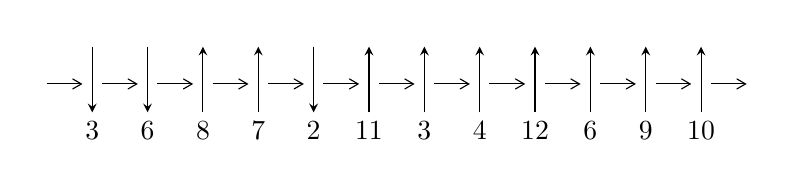
\begin{tikzpicture}[x=20pt, y=17pt]
	% nodes
	\node (C0) at (0, 0) {};
	\node (C1) at (1, 0) {};
	\node (C1U) at (1, +1) {};
	\node (C1D) at (1, -1) {3};

	\node (C2) at (2, 0) {};
	\node (C2U) at (2, +1) {};
	\node (C2D) at (2, -1) {6};

	\node (C3) at (3, 0) {};
	\node (C3U) at (3, +1) {};
	\node (C3D) at (3, -1) {8};

	\node (C4) at (4, 0) {};
	\node (C4U) at (4, +1) {};
	\node (C4D) at (4, -1) {7};

	\node (C5) at (5, 0) {};
	\node (C5U) at (5, +1) {};
	\node (C5D) at (5, -1) {2};

	\node (C6) at (6, 0) {};
	\node (C6U) at (6, +1) {};
	\node (C6D) at (6, -1) {11};

	\node (C7) at (7, 0) {};
	\node (C7U) at (7, +1) {};
	\node (C7D) at (7, -1) {3};

	\node (C8) at (8, 0) {};
	\node (C8U) at (8, +1) {};
	\node (C8D) at (8, -1) {4};

	\node (C9) at (9, 0) {};
	\node (C9U) at (9, +1) {};
	\node (C9D) at (9, -1) {12};

	\node (C10) at (10, 0) {};
	\node (C10U) at (10, +1) {};
	\node (C10D) at (10, -1) {6};

	\node (C11) at (11, 0) {};
	\node (C11U) at (11, +1) {};
	\node (C11D) at (11, -1) {9};

	\node (C12) at (12, 0) {};
	\node (C12U) at (12, +1) {};
	\node (C12D) at (12, -1) {10};
	\node (C13) at (13, 0) {};

	% arrows
	\draw[->,>={angle 60}]
	(C0) edge (C1) (C1) edge (C2) (C2) edge (C3) (C3) edge (C4) (C4) edge (C5) (C5) edge (C6) (C6) edge (C7) (C7) edge (C8) (C8) edge (C9) (C9) edge (C10) (C10) edge (C11) (C11) edge (C12) (C12) edge (C13) ;	\draw[->,>=stealth]
	(C1U) edge (C1D) (C2U) edge (C2D) (C3D) edge (C3U) (C4D) edge (C4U) (C5U) edge (C5D) (C6D) edge (C6U) (C7D) edge (C7U) (C8D) edge (C8U) (C9D) edge (C9U) (C10D) edge (C10U) (C11D) edge (C11U) (C12D) edge (C12U) ;
	\end{tikzpicture} \\
\hhline{~~} \\& 
\textbf{Solving Sequence} \\ \cline{2-2} 
 &
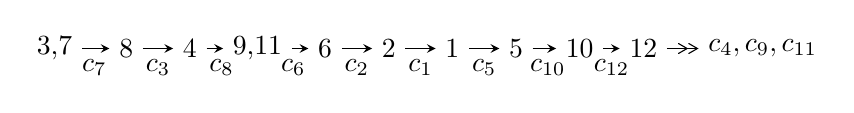
\begin{tikzpicture}[x=23pt, y=7pt]
	% node
	\node (A0) at (-1/8, 0) {3,7};
	\node (A1) at (1, 0) {8};
	\node (A2) at (2, 0) {4};
	\node (A3) at (49/16, 0) {9,11};
	\node (A4) at (33/8, 0) {6};
	\node (A5) at (41/8, 0) {2};
	\node (A6) at (49/8, 0) {1};
	\node (A7) at (57/8, 0) {5};
	\node (A8) at (65/8, 0) {10};
	\node (A9) at (73/8, 0) {12};
	\node (C1) at (1/2, -1) {$c_{7}$};
	\node (C2) at (3/2, -1) {$c_{3}$};
	\node (C3) at (5/2, -1) {$c_{8}$};
	\node (C4) at (29/8, -1) {$c_{6}$};
	\node (C5) at (37/8, -1) {$c_{2}$};
	\node (C6) at (45/8, -1) {$c_{1}$};
	\node (C7) at (53/8, -1) {$c_{5}$};
	\node (C8) at (61/8, -1) {$c_{10}$};
	\node (C9) at (69/8, -1) {$c_{12}$};
	\node (A10) at (11, 0) {$c_{4},c_{9},c_{11}$};

	% edge
	\draw[->,>=stealth]	
	(A0) edge (A1) (A1) edge (A2) (A2) edge (A3) (A3) edge (A4) (A4) edge (A5) (A5) edge (A6) (A6) edge (A7) (A7) edge (A8) (A8) edge (A9) ;
	\draw[->>,>={angle 60}]	
	(A9) edge (A10);
\end{tikzpicture} \\ 

\end{tabular} \\

\footnotetext{
The image of knot diagram is generated by the software ``\textbf{Draw programme}" developed by Andrew Bartholomew(\url{http://www.layer8.co.uk/maths/draw/index.htm\#Running-draw}), where we modified some parts for our purpose(\url{https://github.com/CATsTAILs/LinksPainter}).
}\phantom \\ \newline 
\centering \textbf{Ideals for irreducible components\footnotemark of $X_{\text{par}}$} 
 
\begin{align*}
I^u_{1}&=\langle 
-1.57884\times10^{37} u^{43}+4.19415\times10^{37} u^{42}+\cdots+3.14492\times10^{36} b+2.00463\times10^{38},\\
\phantom{I^u_{1}}&\phantom{= \langle  }5.51340\times10^{37} u^{43}-1.47280\times10^{38} u^{42}+\cdots+3.14492\times10^{36} a-7.82161\times10^{38},\;u^{44}-3 u^{43}+\cdots-36 u+4\rangle \\
I^u_{2}&=\langle 
a u+b+2 a+1,\;2 a^2- a u+2 a+2 u-3,\;u^2-2\rangle \\
\\
I^v_{1}&=\langle 
a,\;b+v-2,\;v^2-3 v+1\rangle \\
\end{align*}
\raggedright * 3 irreducible components of $\dim_{\mathbb{C}}=0$, with total 50 representations.\\
\footnotetext{All coefficients of polynomials are rational numbers. But the coefficients are sometimes approximated in decimal forms when there is not enough margin.}
\newpage
\renewcommand{\arraystretch}{1}
\centering \section*{I. $I^u_{1}= \langle -1.58\times10^{37} u^{43}+4.19\times10^{37} u^{42}+\cdots+3.14\times10^{36} b+2.00\times10^{38},\;5.51\times10^{37} u^{43}-1.47\times10^{38} u^{42}+\cdots+3.14\times10^{36} a-7.82\times10^{38},\;u^{44}-3 u^{43}+\cdots-36 u+4 \rangle$}
\flushleft \textbf{(i) Arc colorings}\\
\begin{tabular}{m{7pt} m{180pt} m{7pt} m{180pt} }
\flushright $a_{3}=$&$\begin{pmatrix}0\\u\end{pmatrix}$ \\
\flushright $a_{7}=$&$\begin{pmatrix}1\\0\end{pmatrix}$ \\
\flushright $a_{8}=$&$\begin{pmatrix}1\\- u^2\end{pmatrix}$ \\
\flushright $a_{4}=$&$\begin{pmatrix}u\\- u^3+u\end{pmatrix}$ \\
\flushright $a_{9}=$&$\begin{pmatrix}- u^2+1\\u^4-2 u^2\end{pmatrix}$ \\
\flushright $a_{11}=$&$\begin{pmatrix}-17.5312 u^{43}+46.8311 u^{42}+\cdots-1316.37 u+248.706\\5.02029 u^{43}-13.3363 u^{42}+\cdots+367.657 u-63.7420\end{pmatrix}$ \\
\flushright $a_{6}=$&$\begin{pmatrix}3.47461 u^{43}-10.7515 u^{42}+\cdots+355.136 u-74.5401\\-1.68885 u^{43}+5.62072 u^{42}+\cdots-173.747 u+30.1506\end{pmatrix}$ \\
\flushright $a_{2}=$&$\begin{pmatrix}-9.86564 u^{43}+26.8155 u^{42}+\cdots-755.031 u+138.369\\-4.70217 u^{43}+10.4432 u^{42}+\cdots-226.148 u+33.6781\end{pmatrix}$ \\
\flushright $a_{1}=$&$\begin{pmatrix}-9.86564 u^{43}+26.8155 u^{42}+\cdots-755.031 u+138.369\\-4.03012 u^{43}+8.38511 u^{42}+\cdots-165.479 u+22.5523\end{pmatrix}$ \\
\flushright $a_{5}=$&$\begin{pmatrix}- u^3+2 u\\- u^3+u\end{pmatrix}$ \\
\flushright $a_{10}=$&$\begin{pmatrix}-19.4067 u^{43}+52.8978 u^{42}+\cdots-1495.34 u+274.133\\-4.36737 u^{43}+8.86394 u^{42}+\cdots-164.017 u+21.4464\end{pmatrix}$ \\
\flushright $a_{12}=$&$\begin{pmatrix}-15.0159 u^{43}+40.6500 u^{42}+\cdots-1164.20 u+225.930\\5.45610 u^{43}-13.6789 u^{42}+\cdots+357.423 u-61.0333\end{pmatrix}$\\&\end{tabular}
\flushleft \textbf{(ii) Obstruction class $= -1$}\\~\\
\flushleft \textbf{(iii) Cusp Shapes $= -58.5401 u^{43}+159.424 u^{42}+\cdots-4534.07 u+846.150$}\\~\\
\newpage\renewcommand{\arraystretch}{1}
\flushleft \textbf{(iv) u-Polynomials at the component}\newline \\
\begin{tabular}{m{50pt}|m{274pt}}
Crossings & \hspace{64pt}u-Polynomials at each crossing \\
\hline $$\begin{aligned}c_{1}\end{aligned}$$&$\begin{aligned}
&u^{44}+45 u^{43}+\cdots+4203 u+81
\end{aligned}$\\
\hline $$\begin{aligned}c_{2},c_{5}\end{aligned}$$&$\begin{aligned}
&u^{44}+3 u^{43}+\cdots+21 u-9
\end{aligned}$\\
\hline $$\begin{aligned}c_{3},c_{7},c_{8}\end{aligned}$$&$\begin{aligned}
&u^{44}-3 u^{43}+\cdots-36 u+4
\end{aligned}$\\
\hline $$\begin{aligned}c_{4}\end{aligned}$$&$\begin{aligned}
&u^{44}+9 u^{43}+\cdots+1500 u-964
\end{aligned}$\\
\hline $$\begin{aligned}c_{6},c_{10}\end{aligned}$$&$\begin{aligned}
&u^{44}+2 u^{43}+\cdots+10 u+1
\end{aligned}$\\
\hline $$\begin{aligned}c_{9},c_{11},c_{12}\end{aligned}$$&$\begin{aligned}
&u^{44}+4 u^{43}+\cdots-18 u+1
\end{aligned}$\\
\hline
\end{tabular}\\~\\
\newpage\renewcommand{\arraystretch}{1}
\flushleft \textbf{(v) Riley Polynomials at the component}\newline \\
\begin{tabular}{m{50pt}|m{274pt}}
Crossings & \hspace{64pt}Riley Polynomials at each crossing \\
\hline $$\begin{aligned}c_{1}\end{aligned}$$&$\begin{aligned}
&y^{44}-85 y^{43}+\cdots-6110883 y+6561
\end{aligned}$\\
\hline $$\begin{aligned}c_{2},c_{5}\end{aligned}$$&$\begin{aligned}
&y^{44}-45 y^{43}+\cdots-4203 y+81
\end{aligned}$\\
\hline $$\begin{aligned}c_{3},c_{7},c_{8}\end{aligned}$$&$\begin{aligned}
&y^{44}-39 y^{43}+\cdots-368 y+16
\end{aligned}$\\
\hline $$\begin{aligned}c_{4}\end{aligned}$$&$\begin{aligned}
&y^{44}+21 y^{43}+\cdots-41187888 y+929296
\end{aligned}$\\
\hline $$\begin{aligned}c_{6},c_{10}\end{aligned}$$&$\begin{aligned}
&y^{44}-12 y^{43}+\cdots-58 y+1
\end{aligned}$\\
\hline $$\begin{aligned}c_{9},c_{11},c_{12}\end{aligned}$$&$\begin{aligned}
&y^{44}-36 y^{43}+\cdots-242 y+1
\end{aligned}$\\
\hline
\end{tabular}\\~\\
\newpage\flushleft \textbf{(vi) Complex Volumes and Cusp Shapes}
$$\begin{array}{c|c|c}  
\text{Solutions to }I^u_{1}& \I (\text{vol} + \sqrt{-1}CS) & \text{Cusp shape}\\
 \hline 
\begin{aligned}
u &= -0.361562 + 0.932667 I \\
a &= \phantom{-}0.23727 - 1.40400 I \\
b &= \phantom{-}0.961486 - 1.024300 I\end{aligned}
 & -4.54866 - 9.17617 I & \phantom{-}5.81808 + 6.48451 I \\ \hline\begin{aligned}
u &= -0.361562 - 0.932667 I \\
a &= \phantom{-}0.23727 + 1.40400 I \\
b &= \phantom{-}0.961486 + 1.024300 I\end{aligned}
 & -4.54866 + 9.17617 I & \phantom{-}5.81808 - 6.48451 I \\ \hline\begin{aligned}
u &= \phantom{-}0.242419 + 0.963914 I \\
a &= \phantom{-}0.542404 + 0.771039 I \\
b &= \phantom{-}0.650253 + 0.479584 I\end{aligned}
 & \phantom{-}2.03227 + 3.85207 I & \phantom{-}10.41827 - 8.61488 I \\ \hline\begin{aligned}
u &= \phantom{-}0.242419 - 0.963914 I \\
a &= \phantom{-}0.542404 - 0.771039 I \\
b &= \phantom{-}0.650253 - 0.479584 I\end{aligned}
 & \phantom{-}2.03227 - 3.85207 I & \phantom{-}10.41827 + 8.61488 I \\ \hline\begin{aligned}
u &= -0.155342 + 0.896950 I \\
a &= -0.31935 + 1.38694 I \\
b &= -0.99704 + 1.03670 I\end{aligned}
 & -8.52514 - 3.75610 I & \phantom{-}2.09209 + 2.89832 I \\ \hline\begin{aligned}
u &= -0.155342 - 0.896950 I \\
a &= -0.31935 - 1.38694 I \\
b &= -0.99704 - 1.03670 I\end{aligned}
 & -8.52514 + 3.75610 I & \phantom{-}2.09209 - 2.89832 I \\ \hline\begin{aligned}
u &= \phantom{-}1.125730 + 0.043899 I \\
a &= \phantom{-}0.058942 + 0.745233 I \\
b &= \phantom{-}0.556341 + 0.553872 I\end{aligned}
 & \phantom{-}1.99922 - 0.04818 I & \phantom{-}6.00000 + 0. I\phantom{ +0.000000I} \\ \hline\begin{aligned}
u &= \phantom{-}1.125730 - 0.043899 I \\
a &= \phantom{-}0.058942 - 0.745233 I \\
b &= \phantom{-}0.556341 - 0.553872 I\end{aligned}
 & \phantom{-}1.99922 + 0.04818 I & \phantom{-}6.00000 + 0. I\phantom{ +0.000000I} \\ \hline\begin{aligned}
u &= -0.851420 + 0.746270 I \\
a &= -0.677609 - 0.190566 I \\
b &= -0.609425 - 0.874938 I\end{aligned}
 & -3.05540 + 3.53185 I & \phantom{-}6.00000 + 0. I\phantom{ +0.000000I} \\ \hline\begin{aligned}
u &= -0.851420 - 0.746270 I \\
a &= -0.677609 + 0.190566 I \\
b &= -0.609425 + 0.874938 I\end{aligned}
 & -3.05540 - 3.53185 I & \phantom{-}6.00000 + 0. I\phantom{ +0.000000I}\\
 \hline 
 \end{array}$$\newpage$$\begin{array}{c|c|c}  
\text{Solutions to }I^u_{1}& \I (\text{vol} + \sqrt{-1}CS) & \text{Cusp shape}\\
 \hline 
\begin{aligned}
u &= \phantom{-}0.060206 + 0.789681 I \\
a &= \phantom{-}0.420124 - 1.337940 I \\
b &= \phantom{-}1.05150 - 1.02729 I\end{aligned}
 & -4.31168 + 1.72166 I & \phantom{-}4.04968 - 1.22187 I \\ \hline\begin{aligned}
u &= \phantom{-}0.060206 - 0.789681 I \\
a &= \phantom{-}0.420124 + 1.337940 I \\
b &= \phantom{-}1.05150 + 1.02729 I\end{aligned}
 & -4.31168 - 1.72166 I & \phantom{-}4.04968 + 1.22187 I \\ \hline\begin{aligned}
u &= -1.104880 + 0.498321 I \\
a &= \phantom{-}0.424315 + 0.083138 I \\
b &= \phantom{-}0.625620 + 1.104260 I\end{aligned}
 & -5.61992 - 1.18304 I & \phantom{-0.000000 } 0 \\ \hline\begin{aligned}
u &= -1.104880 - 0.498321 I \\
a &= \phantom{-}0.424315 - 0.083138 I \\
b &= \phantom{-}0.625620 - 1.104260 I\end{aligned}
 & -5.61992 + 1.18304 I & \phantom{-0.000000 } 0 \\ \hline\begin{aligned}
u &= \phantom{-}1.22068\phantom{ +0.000000I} \\
a &= -1.07819\phantom{ +0.000000I} \\
b &= \phantom{-}1.88874\phantom{ +0.000000I}\end{aligned}
 & \phantom{-}10.3320\phantom{ +0.000000I} & \phantom{-0.000000 } 0 \\ \hline\begin{aligned}
u &= \phantom{-}1.218830 + 0.333934 I \\
a &= \phantom{-}1.13833 - 0.87054 I \\
b &= -1.31850 - 0.66505 I\end{aligned}
 & -0.76043 + 2.33473 I & \phantom{-0.000000 } 0 \\ \hline\begin{aligned}
u &= \phantom{-}1.218830 - 0.333934 I \\
a &= \phantom{-}1.13833 + 0.87054 I \\
b &= -1.31850 + 0.66505 I\end{aligned}
 & -0.76043 - 2.33473 I & \phantom{-0.000000 } 0 \\ \hline\begin{aligned}
u &= -1.271900 + 0.268067 I \\
a &= -0.553133 - 1.124420 I \\
b &= \phantom{-}0.895901 - 0.644934 I\end{aligned}
 & \phantom{-}2.75377 - 4.58010 I & \phantom{-0.000000 } 0 \\ \hline\begin{aligned}
u &= -1.271900 - 0.268067 I \\
a &= -0.553133 + 1.124420 I \\
b &= \phantom{-}0.895901 + 0.644934 I\end{aligned}
 & \phantom{-}2.75377 + 4.58010 I & \phantom{-0.000000 } 0 \\ \hline\begin{aligned}
u &= -1.305420 + 0.064505 I \\
a &= \phantom{-}1.20456 + 0.91583 I \\
b &= -0.813618 + 0.359887 I\end{aligned}
 & \phantom{-}5.20530 - 0.47373 I & \phantom{-0.000000 } 0\\
 \hline 
 \end{array}$$\newpage$$\begin{array}{c|c|c}  
\text{Solutions to }I^u_{1}& \I (\text{vol} + \sqrt{-1}CS) & \text{Cusp shape}\\
 \hline 
\begin{aligned}
u &= -1.305420 - 0.064505 I \\
a &= \phantom{-}1.20456 - 0.91583 I \\
b &= -0.813618 - 0.359887 I\end{aligned}
 & \phantom{-}5.20530 + 0.47373 I & \phantom{-0.000000 } 0 \\ \hline\begin{aligned}
u &= \phantom{-}1.310900 + 0.166284 I \\
a &= -0.028578 + 0.886239 I \\
b &= -0.526233 + 0.907268 I\end{aligned}
 & \phantom{-}5.87917 + 2.87968 I & \phantom{-0.000000 } 0 \\ \hline\begin{aligned}
u &= \phantom{-}1.310900 - 0.166284 I \\
a &= -0.028578 - 0.886239 I \\
b &= -0.526233 - 0.907268 I\end{aligned}
 & \phantom{-}5.87917 - 2.87968 I & \phantom{-0.000000 } 0 \\ \hline\begin{aligned}
u &= -1.310400 + 0.345353 I \\
a &= -0.233101 - 0.138958 I \\
b &= -0.79762 - 1.32164 I\end{aligned}
 & -0.02123 - 5.81626 I & \phantom{-0.000000 } 0 \\ \hline\begin{aligned}
u &= -1.310400 - 0.345353 I \\
a &= -0.233101 + 0.138958 I \\
b &= -0.79762 + 1.32164 I\end{aligned}
 & -0.02123 + 5.81626 I & \phantom{-0.000000 } 0 \\ \hline\begin{aligned}
u &= -1.39785\phantom{ +0.000000I} \\
a &= \phantom{-}8.91764\phantom{ +0.000000I} \\
b &= -0.188474\phantom{ +0.000000I}\end{aligned}
 & \phantom{-}4.90257\phantom{ +0.000000I} & \phantom{-0.000000 } 0 \\ \hline\begin{aligned}
u &= -0.006322 + 0.581193 I \\
a &= -0.89655 - 1.33079 I \\
b &= -0.503249 - 0.484782 I\end{aligned}
 & -1.17226 + 1.37524 I & \phantom{-}0.82630 - 4.37313 I \\ \hline\begin{aligned}
u &= -0.006322 - 0.581193 I \\
a &= -0.89655 + 1.33079 I \\
b &= -0.503249 + 0.484782 I\end{aligned}
 & -1.17226 - 1.37524 I & \phantom{-}0.82630 + 4.37313 I \\ \hline\begin{aligned}
u &= \phantom{-}1.37514 + 0.39616 I \\
a &= -0.881677 + 1.000200 I \\
b &= \phantom{-}1.24438 + 0.87011 I\end{aligned}
 & -3.70647 + 8.39508 I & \phantom{-0.000000 } 0 \\ \hline\begin{aligned}
u &= \phantom{-}1.37514 - 0.39616 I \\
a &= -0.881677 - 1.000200 I \\
b &= \phantom{-}1.24438 - 0.87011 I\end{aligned}
 & -3.70647 - 8.39508 I & \phantom{-0.000000 } 0\\
 \hline 
 \end{array}$$\newpage$$\begin{array}{c|c|c}  
\text{Solutions to }I^u_{1}& \I (\text{vol} + \sqrt{-1}CS) & \text{Cusp shape}\\
 \hline 
\begin{aligned}
u &= \phantom{-}1.33260 + 0.53021 I \\
a &= -0.126765 - 0.487206 I \\
b &= -0.626528 - 0.301390 I\end{aligned}
 & \phantom{-}5.26881 + 2.02524 I & \phantom{-0.000000 } 0 \\ \hline\begin{aligned}
u &= \phantom{-}1.33260 - 0.53021 I \\
a &= -0.126765 + 0.487206 I \\
b &= -0.626528 + 0.301390 I\end{aligned}
 & \phantom{-}5.26881 - 2.02524 I & \phantom{-0.000000 } 0 \\ \hline\begin{aligned}
u &= \phantom{-}1.45079\phantom{ +0.000000I} \\
a &= \phantom{-}0.972042\phantom{ +0.000000I} \\
b &= -0.251576\phantom{ +0.000000I}\end{aligned}
 & \phantom{-}3.37301\phantom{ +0.000000I} & \phantom{-0.000000 } 0 \\ \hline\begin{aligned}
u &= -1.45928\phantom{ +0.000000I} \\
a &= -0.521642\phantom{ +0.000000I} \\
b &= \phantom{-}1.51795\phantom{ +0.000000I}\end{aligned}
 & \phantom{-}13.6404\phantom{ +0.000000I} & \phantom{-0.000000 } 0 \\ \hline\begin{aligned}
u &= -1.41359 + 0.38694 I \\
a &= \phantom{-}0.320048 + 0.993129 I \\
b &= -0.997773 + 0.724464 I\end{aligned}
 & \phantom{-}7.26218 - 8.61162 I & \phantom{-0.000000 } 0 \\ \hline\begin{aligned}
u &= -1.41359 - 0.38694 I \\
a &= \phantom{-}0.320048 - 0.993129 I \\
b &= -0.997773 - 0.724464 I\end{aligned}
 & \phantom{-}7.26218 + 8.61162 I & \phantom{-0.000000 } 0 \\ \hline\begin{aligned}
u &= \phantom{-}1.48503 + 0.37724 I \\
a &= \phantom{-}0.730260 - 1.019420 I \\
b &= -1.20624 - 0.98697 I\end{aligned}
 & \phantom{-}1.34332 + 13.91980 I & \phantom{-0.000000 } 0 \\ \hline\begin{aligned}
u &= \phantom{-}1.48503 - 0.37724 I \\
a &= \phantom{-}0.730260 + 1.019420 I \\
b &= -1.20624 + 0.98697 I\end{aligned}
 & \phantom{-}1.34332 - 13.91980 I & \phantom{-0.000000 } 0 \\ \hline\begin{aligned}
u &= -0.115716 + 0.402697 I \\
a &= -0.38670 + 2.62883 I \\
b &= \phantom{-}0.377022 + 0.479190 I\end{aligned}
 & \phantom{-}1.42746 - 0.71018 I & \phantom{-}6.25077 - 1.25816 I \\ \hline\begin{aligned}
u &= -0.115716 - 0.402697 I \\
a &= -0.38670 - 2.62883 I \\
b &= \phantom{-}0.377022 - 0.479190 I\end{aligned}
 & \phantom{-}1.42746 + 0.71018 I & \phantom{-}6.25077 + 1.25816 I\\
 \hline 
 \end{array}$$\newpage$$\begin{array}{c|c|c}  
\text{Solutions to }I^u_{1}& \I (\text{vol} + \sqrt{-1}CS) & \text{Cusp shape}\\
 \hline 
\begin{aligned}
u &= \phantom{-}0.339286\phantom{ +0.000000I} \\
a &= -1.00783\phantom{ +0.000000I} \\
b &= -1.53932\phantom{ +0.000000I}\end{aligned}
 & \phantom{-}7.49147\phantom{ +0.000000I} & \phantom{-}26.0080\phantom{ +0.000000I} \\ \hline\begin{aligned}
u &= \phantom{-}0.302786\phantom{ +0.000000I} \\
a &= -0.689575\phantom{ +0.000000I} \\
b &= \phantom{-}0.583905\phantom{ +0.000000I}\end{aligned}
 & \phantom{-}0.759214\phantom{ +0.000000I} & \phantom{-}14.0520\phantom{ +0.000000I} \\ \hline\begin{aligned}
u &= \phantom{-}0.266557\phantom{ +0.000000I} \\
a &= \phantom{-}9.48986\phantom{ +0.000000I} \\
b &= -0.525421\phantom{ +0.000000I}\end{aligned}
 & -0.455563\phantom{ +0.000000I} & \phantom{-}39.4620\phantom{ +0.000000I} \\ \hline\begin{aligned}
u &= \phantom{-}1.76844\phantom{ +0.000000I} \\
a &= -0.0279231\phantom{ +0.000000I} \\
b &= \phantom{-}0.581616\phantom{ +0.000000I}\end{aligned}
 & \phantom{-}6.40427\phantom{ +0.000000I} & \phantom{-0.000000 } 0\\
 \hline 
 \end{array}$$\newpage\newpage\renewcommand{\arraystretch}{1}
\centering \section*{II. $I^u_{2}= \langle a u+b+2 a+1,\;2 a^2- a u+2 a+2 u-3,\;u^2-2 \rangle$}
\flushleft \textbf{(i) Arc colorings}\\
\begin{tabular}{m{7pt} m{180pt} m{7pt} m{180pt} }
\flushright $a_{3}=$&$\begin{pmatrix}0\\u\end{pmatrix}$ \\
\flushright $a_{7}=$&$\begin{pmatrix}1\\0\end{pmatrix}$ \\
\flushright $a_{8}=$&$\begin{pmatrix}1\\-2\end{pmatrix}$ \\
\flushright $a_{4}=$&$\begin{pmatrix}u\\- u\end{pmatrix}$ \\
\flushright $a_{9}=$&$\begin{pmatrix}-1\\0\end{pmatrix}$ \\
\flushright $a_{11}=$&$\begin{pmatrix}a\\- a u-2 a-1\end{pmatrix}$ \\
\flushright $a_{6}=$&$\begin{pmatrix}\frac{1}{2} u\\a u+2 a+2\end{pmatrix}$ \\
\flushright $a_{2}=$&$\begin{pmatrix}\frac{1}{2} u\\a u+2 a+u+2\end{pmatrix}$ \\
\flushright $a_{1}=$&$\begin{pmatrix}\frac{1}{2} u\\a u+2 a+2\end{pmatrix}$ \\
\flushright $a_{5}=$&$\begin{pmatrix}0\\- u\end{pmatrix}$ \\
\flushright $a_{10}=$&$\begin{pmatrix}a u+2 a+\frac{1}{2} u\\a u+2 a+2\end{pmatrix}$ \\
\flushright $a_{12}=$&$\begin{pmatrix}- a u- a-1\\- a u-2 a-1\end{pmatrix}$\\&\end{tabular}
\flushleft \textbf{(ii) Obstruction class $= 1$}\\~\\
\flushleft \textbf{(iii) Cusp Shapes $= 12$}\\~\\
\newpage\renewcommand{\arraystretch}{1}
\flushleft \textbf{(iv) u-Polynomials at the component}\newline \\
\begin{tabular}{m{50pt}|m{274pt}}
Crossings & \hspace{64pt}u-Polynomials at each crossing \\
\hline $$\begin{aligned}c_{1},c_{5}\end{aligned}$$&$\begin{aligned}
&(u-1)^4
\end{aligned}$\\
\hline $$\begin{aligned}c_{2}\end{aligned}$$&$\begin{aligned}
&(u+1)^4
\end{aligned}$\\
\hline $$\begin{aligned}c_{3},c_{4},c_{7}\\c_{8}\end{aligned}$$&$\begin{aligned}
&(u^2-2)^2
\end{aligned}$\\
\hline $$\begin{aligned}c_{6},c_{11},c_{12}\end{aligned}$$&$\begin{aligned}
&(u^2+u-1)^2
\end{aligned}$\\
\hline $$\begin{aligned}c_{9},c_{10}\end{aligned}$$&$\begin{aligned}
&(u^2- u-1)^2
\end{aligned}$\\
\hline
\end{tabular}\\~\\
\newpage\renewcommand{\arraystretch}{1}
\flushleft \textbf{(v) Riley Polynomials at the component}\newline \\
\begin{tabular}{m{50pt}|m{274pt}}
Crossings & \hspace{64pt}Riley Polynomials at each crossing \\
\hline $$\begin{aligned}c_{1},c_{2},c_{5}\end{aligned}$$&$\begin{aligned}
&(y-1)^4
\end{aligned}$\\
\hline $$\begin{aligned}c_{3},c_{4},c_{7}\\c_{8}\end{aligned}$$&$\begin{aligned}
&(y-2)^4
\end{aligned}$\\
\hline $$\begin{aligned}c_{6},c_{9},c_{10}\\c_{11},c_{12}\end{aligned}$$&$\begin{aligned}
&(y^2-3 y+1)^2
\end{aligned}$\\
\hline
\end{tabular}\\~\\
\newpage\flushleft \textbf{(vi) Complex Volumes and Cusp Shapes}
$$\begin{array}{c|c|c}  
\text{Solutions to }I^u_{2}& \I (\text{vol} + \sqrt{-1}CS) & \text{Cusp shape}\\
 \hline 
\begin{aligned}
u &= \phantom{-}1.41421\phantom{ +0.000000I} \\
a &= -0.473911\phantom{ +0.000000I} \\
b &= \phantom{-}0.618034\phantom{ +0.000000I}\end{aligned}
 & \phantom{-}4.27683\phantom{ +0.000000I} & \phantom{-}12.0000\phantom{ +0.000000I} \\ \hline\begin{aligned}
u &= \phantom{-}1.41421\phantom{ +0.000000I} \\
a &= \phantom{-}0.181018\phantom{ +0.000000I} \\
b &= -1.61803\phantom{ +0.000000I}\end{aligned}
 & \phantom{-}12.1725\phantom{ +0.000000I} & \phantom{-}12.0000\phantom{ +0.000000I} \\ \hline\begin{aligned}
u &= -1.41421\phantom{ +0.000000I} \\
a &= \phantom{-}1.05505\phantom{ +0.000000I} \\
b &= -1.61803\phantom{ +0.000000I}\end{aligned}
 & \phantom{-}12.1725\phantom{ +0.000000I} & \phantom{-}12.0000\phantom{ +0.000000I} \\ \hline\begin{aligned}
u &= -1.41421\phantom{ +0.000000I} \\
a &= -2.76216\phantom{ +0.000000I} \\
b &= \phantom{-}0.618034\phantom{ +0.000000I}\end{aligned}
 & \phantom{-}4.27683\phantom{ +0.000000I} & \phantom{-}12.0000\phantom{ +0.000000I}\\
 \hline 
 \end{array}$$\newpage\newpage\renewcommand{\arraystretch}{1}
\centering \section*{III. $I^v_{1}= \langle a,\;b+v-2,\;v^2-3 v+1 \rangle$}
\flushleft \textbf{(i) Arc colorings}\\
\begin{tabular}{m{7pt} m{180pt} m{7pt} m{180pt} }
\flushright $a_{3}=$&$\begin{pmatrix}v\\0\end{pmatrix}$ \\
\flushright $a_{7}=$&$\begin{pmatrix}1\\0\end{pmatrix}$ \\
\flushright $a_{8}=$&$\begin{pmatrix}1\\0\end{pmatrix}$ \\
\flushright $a_{4}=$&$\begin{pmatrix}v\\0\end{pmatrix}$ \\
\flushright $a_{9}=$&$\begin{pmatrix}1\\0\end{pmatrix}$ \\
\flushright $a_{11}=$&$\begin{pmatrix}0\\- v+2\end{pmatrix}$ \\
\flushright $a_{6}=$&$\begin{pmatrix}1\\- v+3\end{pmatrix}$ \\
\flushright $a_{2}=$&$\begin{pmatrix}v-1\\v-3\end{pmatrix}$ \\
\flushright $a_{1}=$&$\begin{pmatrix}-1\\v-3\end{pmatrix}$ \\
\flushright $a_{5}=$&$\begin{pmatrix}v\\0\end{pmatrix}$ \\
\flushright $a_{10}=$&$\begin{pmatrix}v-2\\v-3\end{pmatrix}$ \\
\flushright $a_{12}=$&$\begin{pmatrix}- v+2\\- v+2\end{pmatrix}$\\&\end{tabular}
\flushleft \textbf{(ii) Obstruction class $= 1$}\\~\\
\flushleft \textbf{(iii) Cusp Shapes $= -6$}\\~\\
\newpage\renewcommand{\arraystretch}{1}
\flushleft \textbf{(iv) u-Polynomials at the component}\newline \\
\begin{tabular}{m{50pt}|m{274pt}}
Crossings & \hspace{64pt}u-Polynomials at each crossing \\
\hline $$\begin{aligned}c_{1},c_{2}\end{aligned}$$&$\begin{aligned}
&(u-1)^2
\end{aligned}$\\
\hline $$\begin{aligned}c_{3},c_{4},c_{7}\\c_{8}\end{aligned}$$&$\begin{aligned}
&u^2
\end{aligned}$\\
\hline $$\begin{aligned}c_{5}\end{aligned}$$&$\begin{aligned}
&(u+1)^2
\end{aligned}$\\
\hline $$\begin{aligned}c_{6},c_{9}\end{aligned}$$&$\begin{aligned}
&u^2- u-1
\end{aligned}$\\
\hline $$\begin{aligned}c_{10},c_{11},c_{12}\end{aligned}$$&$\begin{aligned}
&u^2+u-1
\end{aligned}$\\
\hline
\end{tabular}\\~\\
\newpage\renewcommand{\arraystretch}{1}
\flushleft \textbf{(v) Riley Polynomials at the component}\newline \\
\begin{tabular}{m{50pt}|m{274pt}}
Crossings & \hspace{64pt}Riley Polynomials at each crossing \\
\hline $$\begin{aligned}c_{1},c_{2},c_{5}\end{aligned}$$&$\begin{aligned}
&(y-1)^2
\end{aligned}$\\
\hline $$\begin{aligned}c_{3},c_{4},c_{7}\\c_{8}\end{aligned}$$&$\begin{aligned}
&y^2
\end{aligned}$\\
\hline $$\begin{aligned}c_{6},c_{9},c_{10}\\c_{11},c_{12}\end{aligned}$$&$\begin{aligned}
&y^2-3 y+1
\end{aligned}$\\
\hline
\end{tabular}\\~\\
\newpage\flushleft \textbf{(vi) Complex Volumes and Cusp Shapes}
$$\begin{array}{c|c|c}  
\text{Solutions to }I^v_{1}& \I (\text{vol} + \sqrt{-1}CS) & \text{Cusp shape}\\
 \hline 
\begin{aligned}
v &= \phantom{-}0.381966\phantom{ +0.000000I} \\
a &= \phantom{-0.000000 } 0 \\
b &= \phantom{-}1.61803\phantom{ +0.000000I}\end{aligned}
 & \phantom{-}7.23771\phantom{ +0.000000I} & -6.00000\phantom{ +0.000000I} \\ \hline\begin{aligned}
v &= \phantom{-}2.61803\phantom{ +0.000000I} \\
a &= \phantom{-0.000000 } 0 \\
b &= -0.618034\phantom{ +0.000000I}\end{aligned}
 & -0.657974\phantom{ +0.000000I} & -6.00000\phantom{ +0.000000I}\\
 \hline 
 \end{array}$$\newpage
\newpage\renewcommand{\arraystretch}{1}
\centering \section*{ IV. u-Polynomials}
\begin{tabular}{m{50pt}|m{274pt}}
Crossings & \hspace{64pt}u-Polynomials at each crossing \\
\hline $$\begin{aligned}c_{1}\end{aligned}$$&$\begin{aligned}
&((u-1)^6)(u^{44}+45 u^{43}+\cdots+4203 u+81)
\end{aligned}$\\
\hline $$\begin{aligned}c_{2}\end{aligned}$$&$\begin{aligned}
&((u-1)^2)(u+1)^4(u^{44}+3 u^{43}+\cdots+21 u-9)
\end{aligned}$\\
\hline $$\begin{aligned}c_{3},c_{7},c_{8}\end{aligned}$$&$\begin{aligned}
&u^2(u^2-2)^2(u^{44}-3 u^{43}+\cdots-36 u+4)
\end{aligned}$\\
\hline $$\begin{aligned}c_{4}\end{aligned}$$&$\begin{aligned}
&u^2(u^2-2)^2(u^{44}+9 u^{43}+\cdots+1500 u-964)
\end{aligned}$\\
\hline $$\begin{aligned}c_{5}\end{aligned}$$&$\begin{aligned}
&((u-1)^4)(u+1)^2(u^{44}+3 u^{43}+\cdots+21 u-9)
\end{aligned}$\\
\hline $$\begin{aligned}c_{6}\end{aligned}$$&$\begin{aligned}
&(u^2- u-1)(u^2+u-1)^2(u^{44}+2 u^{43}+\cdots+10 u+1)
\end{aligned}$\\
\hline $$\begin{aligned}c_{9}\end{aligned}$$&$\begin{aligned}
&((u^2- u-1)^3)(u^{44}+4 u^{43}+\cdots-18 u+1)
\end{aligned}$\\
\hline $$\begin{aligned}c_{10}\end{aligned}$$&$\begin{aligned}
&((u^2- u-1)^2)(u^2+u-1)(u^{44}+2 u^{43}+\cdots+10 u+1)
\end{aligned}$\\
\hline $$\begin{aligned}c_{11},c_{12}\end{aligned}$$&$\begin{aligned}
&((u^2+u-1)^3)(u^{44}+4 u^{43}+\cdots-18 u+1)
\end{aligned}$\\
\hline
\end{tabular}\newpage\renewcommand{\arraystretch}{1}
\centering \section*{ V. Riley Polynomials}
\begin{tabular}{m{50pt}|m{274pt}}
Crossings & \hspace{64pt}Riley Polynomials at each crossing \\
\hline $$\begin{aligned}c_{1}\end{aligned}$$&$\begin{aligned}
&((y-1)^6)(y^{44}-85 y^{43}+\cdots-6110883 y+6561)
\end{aligned}$\\
\hline $$\begin{aligned}c_{2},c_{5}\end{aligned}$$&$\begin{aligned}
&((y-1)^6)(y^{44}-45 y^{43}+\cdots-4203 y+81)
\end{aligned}$\\
\hline $$\begin{aligned}c_{3},c_{7},c_{8}\end{aligned}$$&$\begin{aligned}
&y^2(y-2)^4(y^{44}-39 y^{43}+\cdots-368 y+16)
\end{aligned}$\\
\hline $$\begin{aligned}c_{4}\end{aligned}$$&$\begin{aligned}
&y^2(y-2)^4(y^{44}+21 y^{43}+\cdots-4.11879\times10^{7} y+929296)
\end{aligned}$\\
\hline $$\begin{aligned}c_{6},c_{10}\end{aligned}$$&$\begin{aligned}
&((y^2-3 y+1)^3)(y^{44}-12 y^{43}+\cdots-58 y+1)
\end{aligned}$\\
\hline $$\begin{aligned}c_{9},c_{11},c_{12}\end{aligned}$$&$\begin{aligned}
&((y^2-3 y+1)^3)(y^{44}-36 y^{43}+\cdots-242 y+1)
\end{aligned}$\\
\hline
\end{tabular}
\vskip 2pc
\end{document}